% vim: set spell spelllang=en tw=100 et sw=4 sts=4 foldmethod=marker foldmarker={{{,}}} :

\documentclass{beamer}

\usepackage{tikz}
\usepackage{xcolor}
\usepackage{complexity}
\usepackage{hyperref}
\usepackage{microtype}
\usepackage{amsmath}                   % \operatorname
\usepackage{amsfonts}                  % \mathcal
\usepackage{amssymb}                   % \nexists
\usepackage[vlined]{algorithm2e} % algorithms
\usepackage{centernot}
\usepackage{listings}
\usepackage{csquotes}
\usepackage{fancyvrb}
\usepackage{bussproofs}
\usepackage{multicol}
\usepackage{booktabs}
\usepackage{mathtools}
\usepackage{pifont}
\usepackage{marvosym}

\RequirePackage[tt=false, type1=true]{libertine}
\RequirePackage[varqu]{zi4}
\RequirePackage[libertine]{newtxmath}
\RequirePackage[T1]{fontenc}

\usetikzlibrary{shapes, arrows, shadows, calc, positioning, fit}
\usetikzlibrary{decorations.pathreplacing, decorations.pathmorphing, shapes.misc}
\usetikzlibrary{tikzmark, backgrounds}
\usetikzlibrary{trees, overlay-beamer-styles}

\definecolor{uofguniversityblue}{rgb}{0, 0.219608, 0.396078}
\definecolor{uofgheather}{rgb}{0.356863, 0.32549, 0.490196}
\definecolor{uofgaquamarine}{rgb}{0.603922, 0.72549, 0.678431}
\definecolor{uofgslate}{rgb}{0.309804, 0.34902, 0.380392}
\definecolor{uofgrose}{rgb}{0.823529, 0.470588, 0.709804}
\definecolor{uofgmocha}{rgb}{0.709804, 0.564706, 0.47451}
\definecolor{uofgsandstone}{rgb}{0.321569, 0.278431, 0.231373}
\definecolor{uofgforest}{rgb}{0, 0.2, 0.129412}
\definecolor{uofglawn}{rgb}{0.517647, 0.741176, 0}
\definecolor{uofgcobalt}{rgb}{0, 0.615686, 0.92549}
\definecolor{uofgturquoise}{rgb}{0, 0.709804, 0.819608}
\definecolor{uofgsunshine}{rgb}{1.0, 0.862745, 0.211765}
\definecolor{uofgpumpkin}{rgb}{1.0, 0.72549, 0.282353}
\definecolor{uofgthistle}{rgb}{0.584314, 0.070588, 0.447059}
\definecolor{uofgrust}{rgb}{0.603922, 0.227451, 0.023529}
\definecolor{uofgburgundy}{rgb}{0.490196, 0.133333, 0.223529}
\definecolor{uofgpillarbox}{rgb}{0.701961, 0.047059, 0}
\definecolor{uofglavendar}{rgb}{0.356863, 0.301961, 0.580392}

% {{{ theme things
\useoutertheme[footline=authortitle]{miniframes}
\useinnertheme{rectangles}

\setbeamerfont{block title}{size={}}
\setbeamerfont{title}{size=\large,series=\bfseries}
\setbeamerfont{section title}{size=\large,series=\mdseries}
\setbeamerfont{author}{size=\normalsize,series=\mdseries}
\setbeamercolor*{structure}{fg=uofguniversityblue}
\setbeamercolor*{palette primary}{use=structure,fg=black,bg=white}
\setbeamercolor*{palette secondary}{use=structure,fg=white,bg=uofgcobalt}
\setbeamercolor*{palette tertiary}{use=structure,fg=white,bg=uofguniversityblue}
\setbeamercolor*{palette quaternary}{fg=white,bg=black}

\setbeamercolor*{titlelike}{parent=palette primary}

\beamertemplatenavigationsymbolsempty

\setbeamertemplate{title page}
{
    \begin{tikzpicture}[remember picture, overlay]
        \node at (current page.north west) {
            \begin{tikzpicture}[remember picture, overlay]
                \fill [fill=uofguniversityblue, anchor=north west] (0, 0) rectangle (\paperwidth, -3.0cm);
            \end{tikzpicture}
        };

        \node (logo) [anchor=north east, shift={(-0.6cm,-0.2cm)}] at (current page.north east) {
            \includegraphics[keepaspectratio=true,scale=0.5]{../../images/UoG_keyline.pdf}
        };

        \node (logo2) [anchor=north, below=0.2cm of logo.south] {
            \includegraphics[keepaspectratio=true,scale=0.1]{../../images/RAEngWhite.pdf}
        };

        \coordinate (logos) at ($(logo.south)!0.5!(logo2.north)$);

        \node [anchor=west, xshift=0.2cm] at (current page.west |- logos) {
            \begin{minipage}{0.65\paperwidth}\raggedright
                {\usebeamerfont{title}\usebeamercolor[white]{}\inserttitle}\\[0.5cm]
                {\usebeamerfont{author}\usebeamercolor[white]{}\insertauthor}
            \end{minipage}
        };
    \end{tikzpicture}
}

\setbeamertemplate{section page}
{
    \begin{centering}
        \begin{beamercolorbox}[sep=12pt,center]{part title}
            \usebeamerfont{section title}\insertsection\par
        \end{beamercolorbox}
    \end{centering}
}

\newcommand{\frameofframes}{/}
\newcommand{\setframeofframes}[1]{\renewcommand{\frameofframes}{#1}}

\makeatletter
\setbeamertemplate{footline}
{%
    \begin{beamercolorbox}[colsep=1.5pt]{upper separation line foot}
    \end{beamercolorbox}
    \begin{beamercolorbox}[ht=2.5ex,dp=1.125ex,%
        leftskip=.3cm,rightskip=.3cm plus1fil]{author in head/foot}%
        \leavevmode{\usebeamerfont{author in head/foot}\insertshortauthor}%
        \hfill%
        {\usebeamerfont{institute in head/foot}\usebeamercolor[fg]{institute in head/foot}\insertshortinstitute}%
    \end{beamercolorbox}%
    \begin{beamercolorbox}[ht=2.5ex,dp=1.125ex,%
        leftskip=.3cm,rightskip=.3cm plus1fil]{title in head/foot}%
        {\usebeamerfont{title in head/foot}\insertshorttitle}%
        \hfill%
        {\usebeamerfont{frame number}\usebeamercolor[fg]{frame number}\insertframenumber~\frameofframes~\inserttotalframenumber}
    \end{beamercolorbox}%
    \begin{beamercolorbox}[colsep=1.5pt]{lower separation line foot}
    \end{beamercolorbox}
}

\makeatletter
\newenvironment{nearlyplainframe}[2][]{
    \def\beamer@entrycode{\vspace*{-\headheight}\vspace*{3pt}}
    \setbeamertemplate{headline}
    {%
        \begin{beamercolorbox}[colsep=1.5pt]{upper separation line head}
        \end{beamercolorbox}
        \begin{beamercolorbox}[ht=0.5ex,dp=0.125ex,%
            leftskip=.3cm,rightskip=.3cm plus1fil]{title in head/foot}%
        \end{beamercolorbox}%
        \begin{beamercolorbox}[ht=0.5ex,dp=0.125ex,%
            leftskip=.3cm,rightskip=.3cm plus1fil]{author in head/foot}%
        \end{beamercolorbox}%
        \begin{beamercolorbox}[colsep=1.5pt]{lower separation line head}
        \end{beamercolorbox}
        \vspace*{\headheight}
    }

    \setbeamertemplate{footline}
    {%
        \begin{beamercolorbox}[colsep=1.5pt]{upper separation line foot}
        \end{beamercolorbox}
        \begin{beamercolorbox}[ht=0.5ex,dp=0.125ex,%
            leftskip=.3cm,rightskip=.3cm plus1fil]{author in head/foot}%
        \end{beamercolorbox}%
        \begin{beamercolorbox}[ht=0.5ex,dp=0.125ex,%
            leftskip=.3cm,rightskip=.3cm plus1fil]{title in head/foot}%
        \end{beamercolorbox}%
        \begin{beamercolorbox}[colsep=1.5pt]{lower separation line foot}
        \end{beamercolorbox}
    }

    \begin{frame}[#1]{#2}
    }{
    \end{frame}
}
\makeatother

\makeatletter
\newenvironment{justborderframe}[2][]{
    \def\beamer@entrycode{\vspace*{-\headheight}}
    \setbeamertemplate{headline}
    {%
        \begin{beamercolorbox}[colsep=1.5pt]{upper separation line head}
        \end{beamercolorbox}
        \begin{beamercolorbox}[ht=0.5ex,dp=0.125ex,%
            leftskip=.3cm,rightskip=.3cm plus1fil]{title in head/foot}%
        \end{beamercolorbox}%
        \begin{beamercolorbox}[ht=0.5ex,dp=0.125ex,%
            leftskip=.3cm,rightskip=.3cm plus1fil]{author in head/foot}%
        \end{beamercolorbox}%
        \begin{beamercolorbox}[colsep=1.5pt]{lower separation line head}
        \end{beamercolorbox}
        \vspace*{\headheight}
    }

    \setbeamertemplate{footline}
    {%
        \begin{beamercolorbox}[colsep=1.5pt]{upper separation line foot}
        \end{beamercolorbox}
        \begin{beamercolorbox}[ht=0.5ex,dp=0.125ex,%
            leftskip=.3cm,rightskip=.3cm plus1fil]{author in head/foot}%
        \end{beamercolorbox}%
        \begin{beamercolorbox}[ht=0.5ex,dp=0.125ex,%
            leftskip=.3cm,rightskip=.3cm plus1fil]{title in head/foot}%
        \end{beamercolorbox}%
        \begin{beamercolorbox}[colsep=1.5pt]{lower separation line foot}
        \end{beamercolorbox}
    }

    \begin{frame}[#1]{}
    }{
    \end{frame}
}
\makeatother


% }}}

\author{Ciaran McCreesh}
\title{Is Your Combinatorial Search Algorithm Telling the Truth?}

\begin{document}

{
    \usebackgroundtemplate{
        \tikz[overlay, remember picture]
        \node[at=(current page.south), anchor=south, inner sep=0pt]{\includegraphics[keepaspectratio=true, height=\paperheight]{../../images/background.jpg}};
    }
    \begin{frame}[plain,noframenumbering]
        \titlepage
    \end{frame}
}

\section{Practical Subgraph-Finding Algorithms}

\begin{frame}{The Algorithms I Work On}
\end{frame}

\begin{frame}{Constraint Programming}
\end{frame}

\begin{frame}{Worst-Case Complexity vs Practice}
\end{frame}

\begin{frame}{The Slight Problem\ldots}
\end{frame}

\begin{frame}{How We Fix This}
\end{frame}

\section{Proof Logging}

\begin{frame}{What Is A Proof?}
    \begin{center}
        \includegraphics[keepaspectratio=true,scale=0.30]{shortest-math-paper.jpg}
    \end{center}
\end{frame}

\begin{frame}{Constraints and Satisfiability}
\end{frame}

\begin{frame}{Resolution Proofs}
    \only<1>{
    \begin{minipage}[c]{0.25\framewidth}
        \textcolor{uofgcobalt}{\textbf{Model axioms}}
    \end{minipage}\hfill\begin{minipage}[c]{0.70\framewidth}
        \centering From the input
    \end{minipage}\bigskip

    \begin{minipage}[c]{0.25\framewidth}
        \textcolor{uofgcobalt}{\textbf{Resolution}}
    \end{minipage}\hfill\begin{minipage}[c]{0.70\framewidth}\begin{prooftree}
        \AxiomC{$\textcolor{uofglawn}{x_1} \vee \textcolor{uofglawn}{x_2} \vee \ldots \vee
        \textcolor{uofglawn}{x_i} \vee \textcolor{uofgpillarbox}{c}$}
        \AxiomC{$\textcolor{uofgpillarbox}{\overline{c}} \vee \textcolor{uofgcobalt}{y_1} \vee
        \textcolor{uofgcobalt}{y_2} \vee \ldots \textcolor{uofgcobalt}{y_j}$}
        \BinaryInfC{$\textcolor{uofglawn}{x_1} \vee \textcolor{uofglawn}{x_2} \vee \ldots \vee
        \textcolor{uofglawn}{x_i} \vee \textcolor{uofgcobalt}{y_1} \vee
        \textcolor{uofgcobalt}{y_2} \vee \ldots \vee \textcolor{uofgcobalt}{y_j}$}
    \end{prooftree}\end{minipage}

    \bigskip

    \begin{itemize}
        \item To prove unsatisfiability: resolve until you reach the empty clause.
    \end{itemize}
}
    \only<2->{
        \begin{minipage}[c]{0.30\framewidth}
            \begin{align}
                & x \vee y \vee z \\
                & \overline{x} \vee \overline{y} \vee \overline{z} \\
                & \overline{x} \vee y \\
                & \overline{x} \vee z \\
                & x \vee \overline{y} \\
                & x \vee \overline{z}
            \end{align}
        \end{minipage}\hfill\begin{minipage}[c]{0.60\framewidth}
            \begin{align}
                & 1, 5 \operatorname{on} y && x \vee z \\
                & 6, 7 \operatorname{on} z && x \\
                & 3, 8 \operatorname{on} x && y \\
                & 4, 8 \operatorname{on} x && z \\
                & 2, 8 \operatorname{on} x && \overline{y} \vee \overline{z} \\
                & 9, 11 \operatorname{on} y && \overline{z} \\
                & 10, 12 \operatorname{on} z && \emptyset
            \end{align}

        \end{minipage}
    }
\end{frame}

\begin{frame}{Equisatisfiability and Completeness}
    \begin{itemize}
        \item Start with the constraints we're given.
        \item At each step in a proof, add a new constraint which obviously doesn't affect satisfiability.
        \item If we can derive contradiction, there were no solutions to the original problem.
        \item Using resolution, we can always do this for any unsatisfiable SAT problem.
    \end{itemize}
\end{frame}

\begin{frame}{Reverse Unit Propagation Proofs}
    \begin{itemize}
        \item Unit propagation:
            \begin{itemize}
                \item Look for a clause containing just one literal $\ell$.
                \item Delete $\overline{\ell}$ from every other clause.
                \item Repeat until you can't do anything.
            \end{itemize}
        \item Reverse unit propagation:
            \begin{itemize}
                \item Add the negation of a constraint $C$, and unit propagate.
                \item If contradiction is reached, derive $C$.
            \end{itemize}
        \item Can rewrite to resolution in polynomial time.
    \end{itemize}
\end{frame}

\begin{frame}{Backtracking Search as RUP}
    \only<1>{
        \begin{itemize}
            \item Every time you backtrack, output a RUP step for the sequence of guesses you just
                made.
        \end{itemize}
    }
    \only<2->{
        \setcounter{equation}{0}
        \begin{minipage}[t]{0.30\framewidth}
            \begin{align}
                & x \vee y \vee z \\
                & \overline{x} \vee \overline{y} \vee \overline{z} \\
                & \overline{x} \vee y \\
                & \overline{x} \vee z \\
                & x \vee \overline{y} \\
                & x \vee \overline{z}
            \end{align}
        \end{minipage}\hfill\begin{minipage}[t]{0.60\framewidth}
            \only<3->{
            \begin{align}
                \operatorname{RUP} x &&&\phantom{ \overline{x} \operatorname{assumed} }
                \only<4>{
                    \\
                \nonumber &&& \overline{x} \operatorname{assumed} \\
                \nonumber &&& \overline{y} \operatorname{from} 5 \\
                \nonumber &&& \overline{z} \operatorname{from} 6 \\
                \nonumber &&& x \operatorname{from} 1
            }
                \only<5->{
                    \\
                \operatorname{RUP} \overline{x} &&&
                \only<6>{
                    \\
                \nonumber &&& x \operatorname{assumed} \\
                \nonumber &&& y \operatorname{from} 3 \\
                \nonumber &&& z \operatorname{from} 4 \\
                \nonumber &&& \overline{x} \operatorname{from} 2
            }
            }
                \only<7->{
                \\
                \operatorname{RUP} \emptyset &&&
                \only<8>{
                    \\
                \nonumber &&& x \operatorname{from} 7 \\
                \nonumber &&& \overline{x} \operatorname{from} 8
            }
        }
            \end{align}}

        \end{minipage}
    }
\end{frame}

\begin{frame}{Resolution Can't Count}
\end{frame}

\begin{frame}{Cutting Planes}
\end{frame}

\begin{frame}{Bounds}
\end{frame}

\begin{frame}{Degree Reasoning}
\end{frame}

\begin{frame}{Cardinality Reasoning}
\end{frame}

\begin{frame}{Reformulation}
\end{frame}

\begin{frame}{Non-Implicational Proofs}
\end{frame}

\section{Challenges}

\begin{frame}{What Reasoning Can We Justify?}
\end{frame}

\begin{frame}{Verifed Encodings}
\end{frame}

\begin{frame}{Proof Trimming}
\end{frame}

\begin{frame}{Counting and Sampling without Enumerating}
\end{frame}

\begin{frame}{Going the Other Way}
\end{frame}

\begin{frame}{Getting Involved}
\end{frame}

{
    \usebackgroundtemplate{
        \tikz[overlay, remember picture]
        \node[at=(current page.south), anchor=south, inner
        sep=0pt]{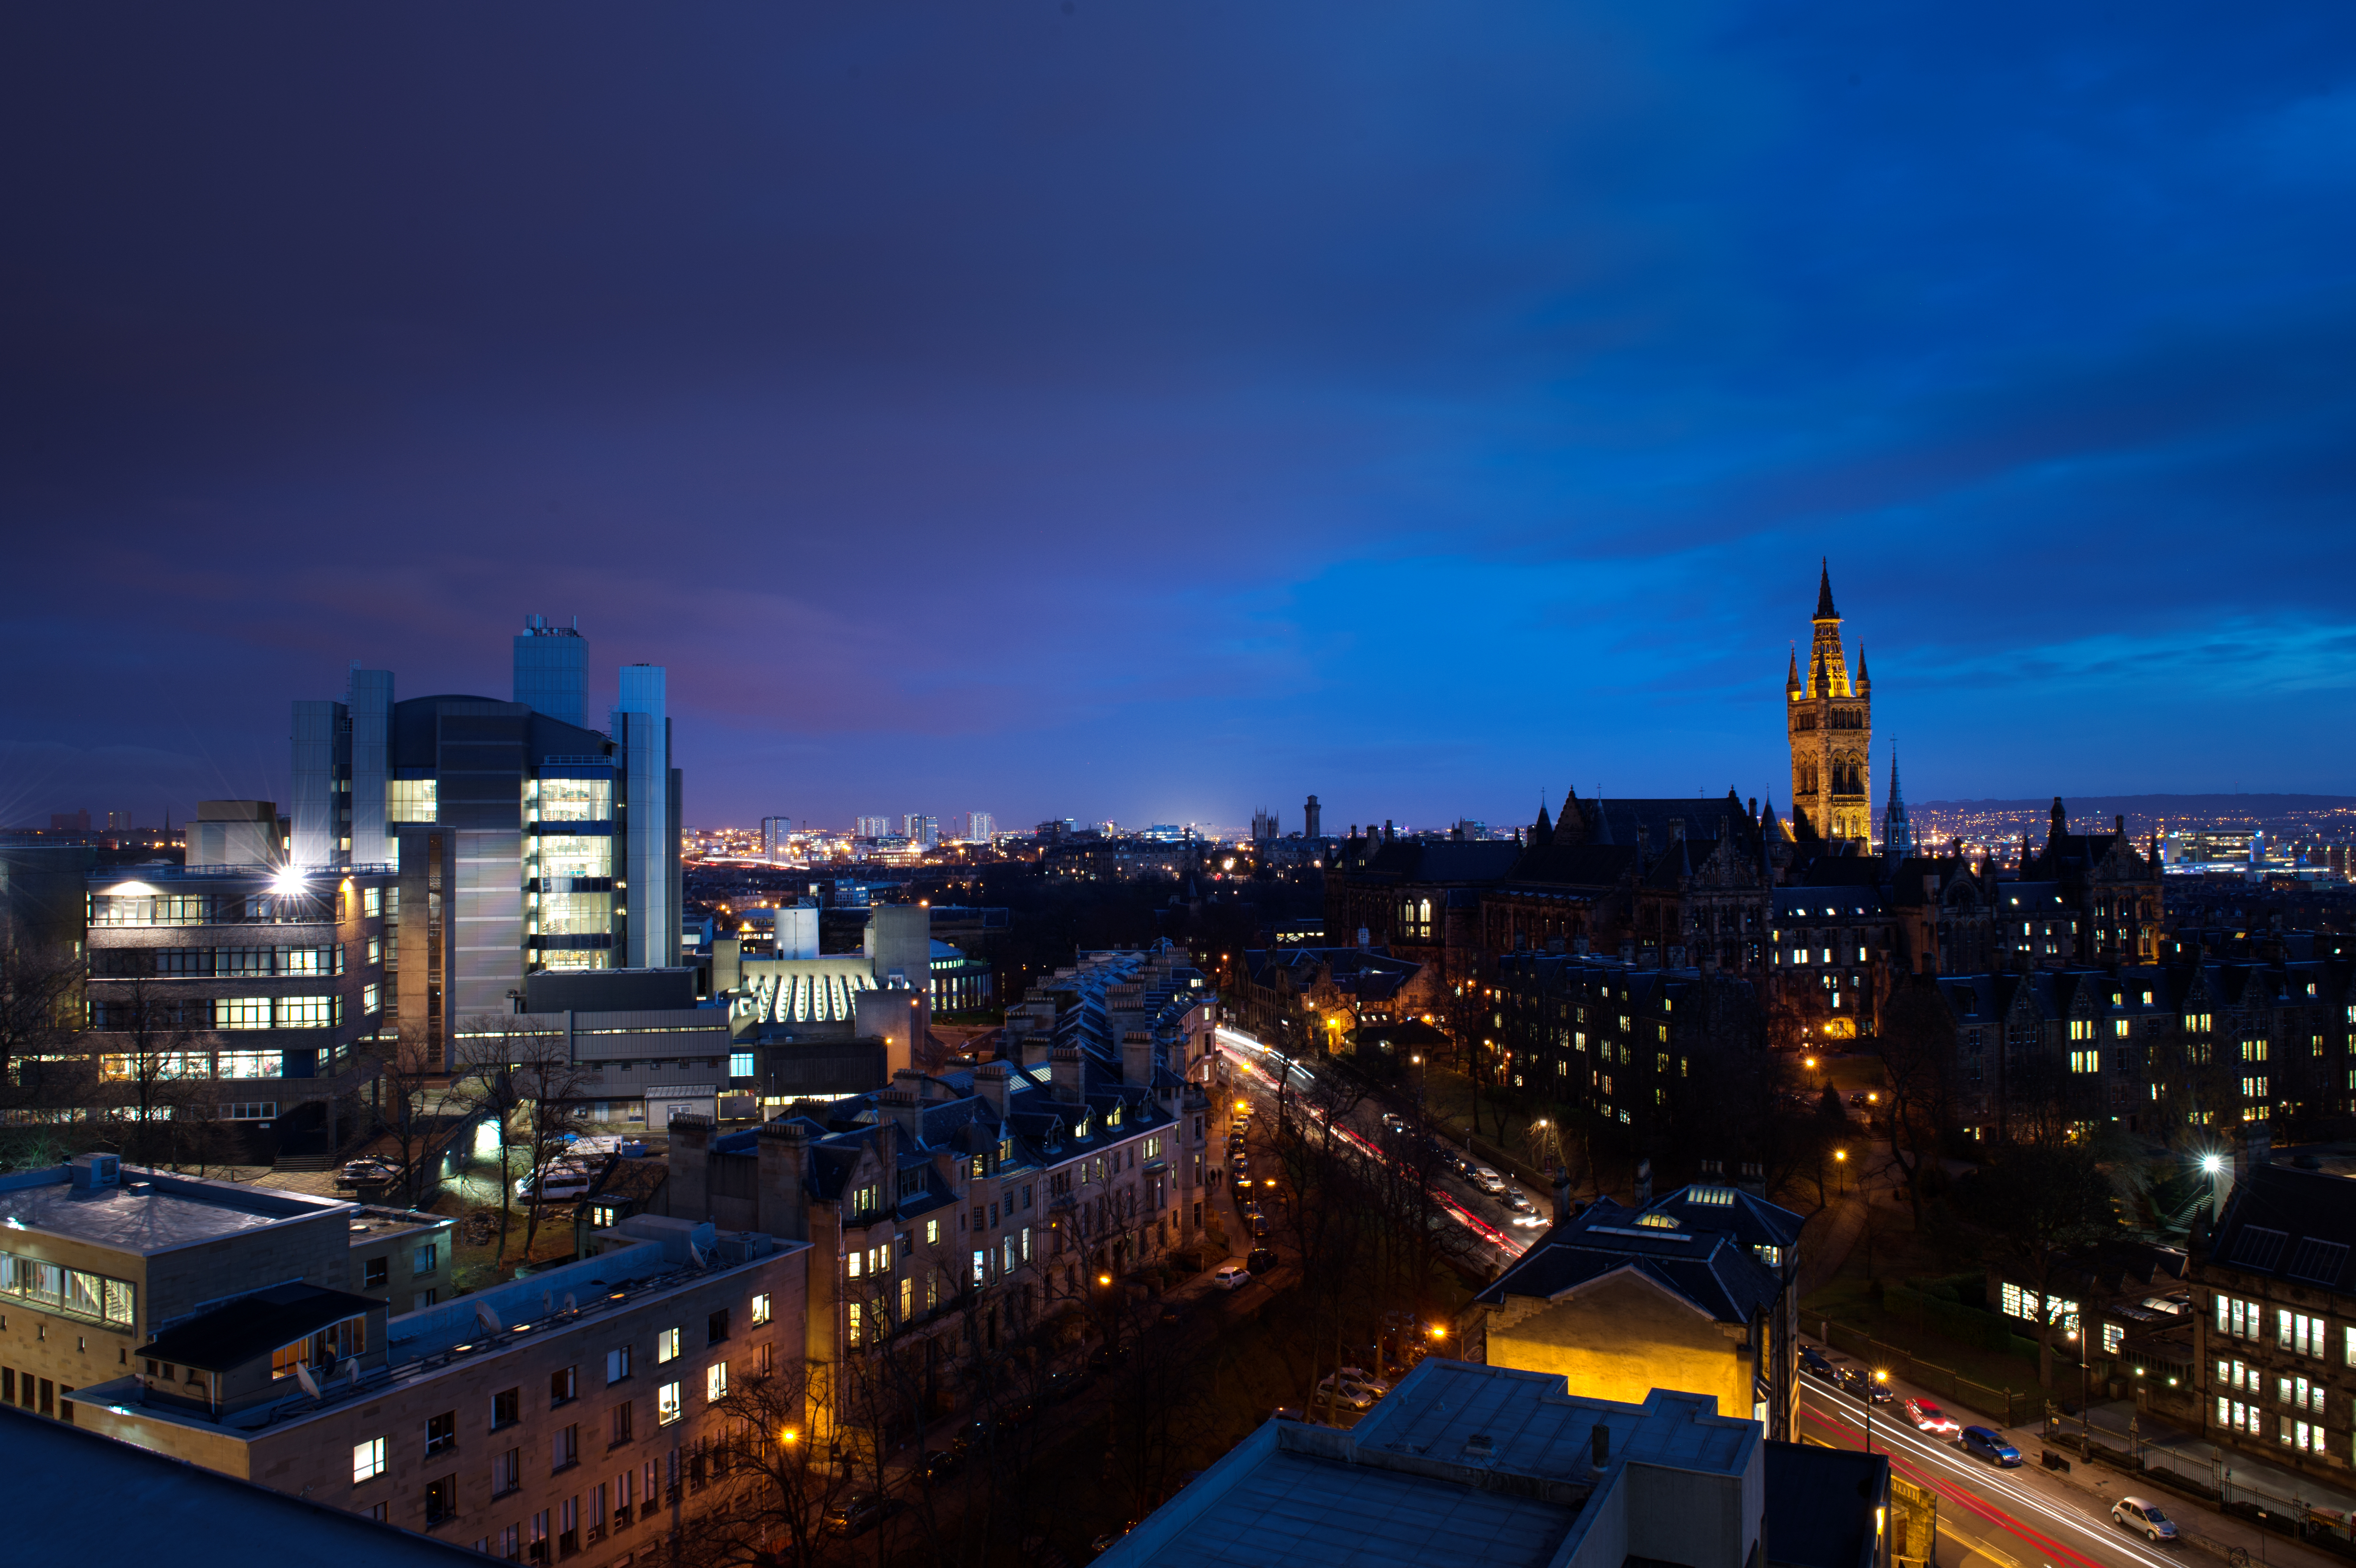
\includegraphics[keepaspectratio=true, width=\paperwidth]{../../images/background2.jpg}};
    }

    \begin{frame}[plain,noframenumbering]
        \begin{tikzpicture}[remember picture, overlay]
            \node at (current page.north west) {
                \begin{tikzpicture}[remember picture, overlay]
                    \fill [fill=uofguniversityblue, anchor=north west] (0, 0) rectangle (\paperwidth, -2.8cm);
                \end{tikzpicture}
            };

            \node (logo) [anchor=north east, shift={(-0.6cm,-0.2cm)}] at (current page.north east) {
                \includegraphics[keepaspectratio=true,scale=0.5]{../../images/UoG_keyline.pdf}
            };

            \node (logo2) [anchor=north, below=0.2cm of logo.south] {
                \includegraphics[keepaspectratio=true,scale=0.1]{../../images/RAEngWhite.pdf}
            };

            \coordinate (logos) at ($(logo.south)!0.5!(logo2.north)$);

            \node [anchor=west, xshift=0.2cm] at (current page.west |- logos) {
                \begin{minipage}{0.60\paperwidth}\raggedright
                    \textcolor{white}{\url{https://ciaranm.github.io/}} \\[0.3cm]
                    \textcolor{white}{\href{mailto:ciaran.mccreesh@glasgow.ac.uk}{\nolinkurl{ciaran.mccreesh@glasgow.ac.uk}}}
                \end{minipage}
            };
        \end{tikzpicture}
    \end{frame}
}

\end{document}

